\section{Application to proplyd bowshocks}
\label{sec:application}

Proplyds are comet-like structures observed in HII regions like Orion Nebula Cluster (ONC). 
These objects are interpreted as a D-type Ionization Front (IF) of a photoevaporated flow 
originated in the protoplanetary disk of a nearby low mass YSO \citep{Johnstone:1998}.
The presure of the surrounding gas is not enough to confine this flow \citep{HA:1998}
may be formed by the interaction of the photoevaporated wind of the proplyds with the stellar wind of $\theta^1~C~Ori$, which is highly supersonic $(M \sim 100)$. 

The density distribution of the photoevaporated flow can be determined using the steady state continuity equation and assuming that almost all ionizing photons are absorbed at the IF \citep{HA:1998} and ignoring dust absorption, can be found that

\begin{align}
N(r_{IF},\theta) = N_0 \cos^{0.5}\theta
\label{eq:nprop}
\end{align}

This scenario can be described with the formalism of \citep{Canto:1996}, who proposes an algebraic solution for the two winds interaction problem in the thin shell approximation. See figure.

\begin{figure}
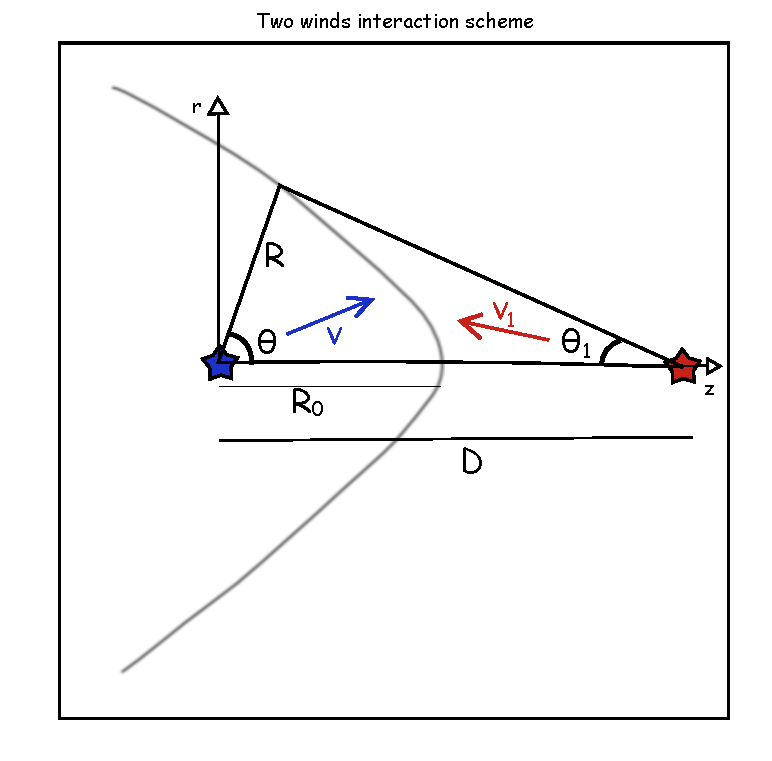
\includegraphics[width=\linewidth]{2winds-scheme}
\caption{Schematic representation of the two winds problem. Any point in the shell is located with the coordinates
$(R,\theta)$, and $\theta_1$ is measured from the external wind position}
\label{fig:2-winds}
\end{figure}

 Combining equations (6),(9)-(11) and (19)-(23) from \citep{Canto:1996} and (\ref{eq:nprop}), we can solve numerically for $R(\theta)$, as shown in figure (add figure later). Also we can
obtain a relation between $\theta$ and $\theta_1$

\begin{align}
\theta_1\cot\theta_1 = 1+ 2\beta I(\theta)\cot\theta - \frac{4}{5}\beta\left(1-\cos^{5/2}\theta\right)
\label{eq:th1th}
\end{align}

\subsection{Characteristic Radii}

$R_0$ is obtained directly from equation () of \citep{Canto:1996} as the distance from the inner source where the RAM pressure of the interacting winds is in equilibrium.

Combinig equation (23) from \citep{Canto:1996} and  (\ref{eq:th1th}) evaluated at $\theta=\frac{\pi}{2}$, we can obtain $R_{90}$ 

\begin{align}
R_{90} \simeq \frac{\left(2.4\beta\right)^{1/2}}{1-0.8\beta}
\label{eq:r90}
\end{align}
%%% Local Variables:
%%% mode: latex
%%% TeX-master: "proplyd-bowshocks"
%%% End:
